\documentclass{standalone}

\usepackage{tikz}
\usetikzlibrary{shapes.geometric}
\begin{document}
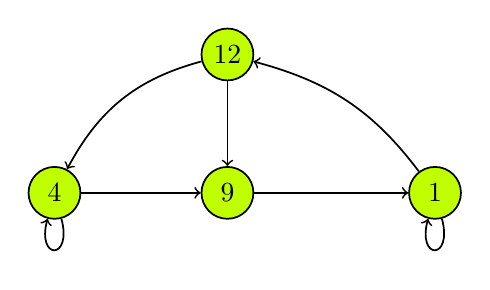
\begin{tikzpicture}
[every node/.style={inner sep=0pt}]
\node (4) [circle, minimum size=18.75pt, fill=lime, line width=0.625pt, draw=black] at (37.5pt, -75.0pt) {\textcolor{black}{4}};
\node (1) [circle, minimum size=18.75pt, fill=lime, line width=0.625pt, draw=black] at (175.0pt, -75.0pt) {\textcolor{black}{1}};
\node (12) [circle, minimum size=18.75pt, fill=lime, line width=0.625pt, draw=black] at (100.0pt, -25.0pt) {\textcolor{black}{12}};
\node (9) [circle, minimum size=18.75pt, fill=lime, line width=0.625pt, draw=black] at (100.0pt, -75.0pt) {\textcolor{black}{9}};
\draw [line width=0.625, ->, color=black, loop below] (4) to (4);
\draw [line width=0.625, ->, color=black, loop below] (1) to (1);
\draw [line width=0.625, ->, color=black] (4) to  (9);
\draw [line width=0.625, ->, color=black] (9) to  (1);
\draw [line width=0.625, ->, color=black] (12) to  (9);
\draw [line width=0.625, ->, color=black] (12) to  [in=62, out=195] (4);
\draw [line width=0.625, ->, color=black] (1) to  [in=345, out=127] (12);
\end{tikzpicture}
\end{document}
